%\documentclass[mathserif]{beamer}
\documentclass[handout]{beamer}
%\usetheme{Goettingen}
\usetheme{Warsaw}
%\usetheme{Singapore}
%\usetheme{Frankfurt}
%\usetheme{Copenhagen}
%\usetheme{Szeged}
%\usetheme{Montpellier}
%\usetheme{CambridgeUS}
%\usecolortheme{}
%\setbeamercovered{transparent}
\usepackage[english, activeacute]{babel}
\usepackage[utf8]{inputenc}
\usepackage{amsmath, amssymb}
\usepackage{dsfont}
\usepackage{graphics}
\usepackage{cases}
\usepackage{graphicx}
\usepackage{pgf}
\usepackage{epsfig}
\usepackage{amssymb}
\usepackage{multirow}	
\usepackage{amstext}
\usepackage[ruled,vlined,lined]{algorithm2e}
\usepackage{amsmath}
\usepackage{epic}
\usepackage{epsfig}
\usepackage{fontenc}
\usepackage{framed,color}
\usepackage{palatino, url, multicol}
\usepackage{listings}
%\algsetup{indent=2em}
\newcommand{\factorial}{\ensuremath{\mbox{\sc Factorial}}}
\newcommand{\BIGOP}[1]{\mathop{\mathchoice%
{\raise-0.22em\hbox{\huge $#1$}}%
{\raise-0.05em\hbox{\Large $#1$}}{\hbox{\large $#1$}}{#1}}}
\newcommand{\bigtimes}{\BIGOP{\times}}
\vspace{-0.5cm}
\title{Introduction to Statistical Inference}
\vspace{-0.5cm}
\author[Felipe Bravo Márquez]{\footnotesize
%\author{\footnotesize  
 \textcolor[rgb]{0.00,0.00,1.00}{Felipe José Bravo Márquez}} 
\date{ \today }


\begin{document}
\begin{frame}
\titlepage


\end{frame}


%%%%%%%%%%%%%%%%%%%%%%%%%%%

% Useful references: http://www.buders.com/UNIVERSITE/Universite_Dersleri/istatistik/sampling_distributions_and_point_estimation_of_parameters.pdf
% http://homepage.divms.uiowa.edu/~rdecook/stat2020/notes/ch7_pt1.pdf

\begin{frame}{Populations and Samples}
\scriptsize{
\begin{itemize}
 
 \item The main goal of statistical inference is investigate properties about a target \textbf{population}.
 
 \item A \textbf{population} is the entire group of individuals that we are interested in studying.
 \item  This could be anything from all humans to a specific type of cell.
 
 \item The individual elements of the population sometimes are  called \textbf{units}.



 \item Example: What is the average height of all people in Chile? Here the population is all the inhabitants of Chile. 
 
 
 \item In order to draw conclusions about a \textbf{population}, it is generally not feasible to gather all the data about it.
 
 \item The special case where you collect data on the entire population is a \textbf{census}.

\end{itemize}

} 
\end{frame}



\begin{frame}{Populations and Samples}
\scriptsize{
\begin{itemize}
 \item In statisical inference we try to make reasonable conclusions about a population based on the evidence provided by \textbf{sample data}.

 
 \item A \textbf{sample staticic} or simply \textbf{statistic} is a quantitative measure calculated from a sample. Examples: the mean, the standard deviation, the minimum, the maximum.
 
 

\end{itemize}

\begin{block}{Example}
\begin{itemize}

\item  Taking a sample \textbf{survey} can help you determine the percentage of people in a population who have a particular characteristic.

 \item Nielsen Media Research takes a \textbf{survey} so they can get an estimate of the proportion of all U.S. households that are tuned to a particular television program  \cite{watkins2010statistics}.
 
\item The true proportion that Nielsen would get from a survey of \textbf{every} household is called a \textbf{population parameter}.

\item Nielsen uses the proportion in the \textbf{sample} as an
\textbf{estimate} of this parameter. 

\item Such an estimate from a sample is called a \textbf{statistic}.
 
\end{itemize}

 
\end{block}


} 
\end{frame}



\begin{frame}{Sampling Methods}
\scriptsize{


\begin{itemize}


 \item Our goal in sampling is to determine the value of a statistic for an entire population of interest, using just a small subset of the population.
 
\item We do this primarily to save time and effort.

\item A good sample is \textbf{representative}: it looks like a small version of the population.


\item A sampling method is \textbf{biased} if it produces samples such that the estimate from the sample is larger or smaller, on average, than the population parameter being estimated.


\item In practice, we can't tell if if a sample is representative, since we can't get all the population data.

\item But, we can tell whether a \textbf{sampling method} is good or not.


\item The problems or \textbf{biases} of a sampling method can come from two sources: 

\begin{enumerate}
\scriptsize{
 \item \textbf{Sampling selection bias}: the method of taking the sample.
 \item \textbf{Response bias}: the method for getting a response.
 }
 \end{enumerate}


\end{itemize}




} 
\end{frame}




\begin{frame}{Sample selection bias}
\scriptsize{

Sample selection bias happens when samples tend to result in estimates of population parameters that systematically are too high or too low \cite{watkins2010statistics}. \\ It can occur in the following ways:
\begin{itemize}


 \item  \textbf{Size bias}: using a method that gives larger units a bigger change of being in the sample. 
 \begin{itemize}
 \scriptsize{
  \item Example: patients who spent more days in a hospital are more likely to be selected for the sample.}
 \end{itemize}

 
 
 
 \item \textbf{Voluntary response bias}: letting people volunteer to be in the sample. 
 \begin{itemize}
 \scriptsize{
  \item  Example:  When a radio program asks people to call in and take sides on some issue, those who care about the issue will be overrepresented, and those who don't care as much might not be represented at all.}
 \end{itemize}


 
 \item \textbf{Convenience sample bias}: units are chosen because of convenience.
 \begin{itemize}
 \scriptsize{
  \item  Example: What percentage of the students in your graduating class plan to go to work immediately after graduation? 
  \item You can use your friends as a quicker and more convenient sample, but almost certainly biased because your friends are likely to have similar plans to yours.}
 \end{itemize}

\end{itemize}


} 
\end{frame}





\begin{frame}{Sample selection bias}
\scriptsize{


\begin{itemize}
 
 \item \textbf{Judgment sampling bias}: selecting the sampling units based on ``expert'' judgment. Problem: experts might overlook important features of a population.
 
 \begin{itemize}
  \scriptsize{
  \item Example: In the early days of US election polling, local ``experts'' were hired to sample voters in their locale by filling certain quotas (so many men, so many women, so many voters over the age of 40, so many employed workers, and so on). 
  \item The poll takers used their own judgment as to whom they selected for the poll. 
  \item It took a very close election (the 1948 presidential election, in which polls were wrong in their prediction) for the polling organizations to realize that quota sampling was a biased method.}
 \end{itemize}



\end{itemize}


} 
\end{frame}




\begin{frame}{Sample selection bias}
\scriptsize{


\begin{itemize}
 
 \item \textbf{Sampling frame bias}: a sampling frame is the ``list'' of all population units from which you select the sample. Constructing an inadequate sampling frame is a cause of bias. 
 
 \begin{itemize}
 \scriptsize{
  \item The problem is that in many problems is extremely hard to make that ``list''. 
  \item How would you list all the people using the Internet worldwide or all the ants in a park? 
  \item For all practical purposes, you can't.
  \item There will often be a difference between the population and the sampling frame.
  \item A sample might represent the units in the frame quite well, but how well your sample represents the population depends on how well you've chosen your frame.
  \item If you start from a bad frame, even the best sampling methods can't save you: bad frame, bad sample \cite{watkins2010statistics}.
 }
 \end{itemize}



\end{itemize}


} 
\end{frame}



\begin{frame}{Response bias}
\scriptsize{
These types of bias derive from the method of obtaining the response.

\begin{itemize}
 \item \textbf{Nonresponse bias}: people often refuse to respond to a survey. These people may be different from those who agree to participate.
 
 \item \textbf{Incorrent response or measurement bias}: the bias might be the result of intentional lying, or come from inaccurate measuring devices, including inaccurate memories of people being interviewed in self-reported data.
 \begin{itemize}
 \begin{scriptsize}
    \item Example 1: many people don't want to admit that they watch a certain television program.
  \item Example 2: patients in medical studies are prone to overstate how well they have followed the physician's orders.
  \item Example 3: many people tend to underestimate the amount of time they actually spend with their cell phones.
 \end{scriptsize}
 \end{itemize}

 
 
\end{itemize}


} 
\end{frame}




\begin{frame}{Response bias}
\scriptsize{

\begin{itemize}

 \item \textbf{Questionnaire bias}: people's opinions may vary depending on the interviewer's tone of voice, the order in which the questions are asked and the wording of the questions, etc..
 
 \begin{itemize}
 \scriptsize{
  \item  Example: Reader's Digest asked the same 1031 people to respond to these two statements:
   \begin{enumerate}
 \scriptsize{

  \item I would be disappointed if Congress cut its funding for public television.
  
  \item Cuts in funding for public television are justified as part of an overall effort to reduce federal spending.
 }
 \end{enumerate}
  \item Note that agreeing with the first statement is pretty much the same as disagreeing with the second. However:
  
  \item First statement: 54\% agreed, 40\% disagreed, and 6\% didn't know.
  \item Second statement: 52\% agreed , 37\% disagreed, and 10\% didn’t know. \cite{barnes1995can}
  
  }
 \end{itemize}

 
\end{itemize}


} 
\end{frame}


\begin{frame}{Random Samples}
\scriptsize{

\begin{itemize}

 \item The key idea for building a good sample is to \textbf{randomize}, that is, let chance choose the sampling units.
 \item Selecting your sample by chance is the only method guaranteed to be unbiased.
\end{itemize}


\begin{block}{Simple Random Sampling}
 \begin{itemize}
 \item All possible samples of a given fixed size are equally likely.
 \item All individuals in the population are indexed and randomly drawn with equal probability until the sample size is reached.
\end{itemize}
\end{block}


\begin{block}{Stratified Random Sampling}
 \begin{itemize}
 \item We divide the population into subgroups based on shared characteristics (e.g., country, city) that do not overlap and that cover the entire sampling frame.
 \item These subgroups are called strata.
 \item Take a simple random sample for each strata proportional to its size.
 \item It ensures that every strata is properly represented in the sample.
\end{itemize}
\end{block}





} 
\end{frame}


\begin{frame}{Random Samples}
\scriptsize{

\begin{figure}[h!]
	\centering
	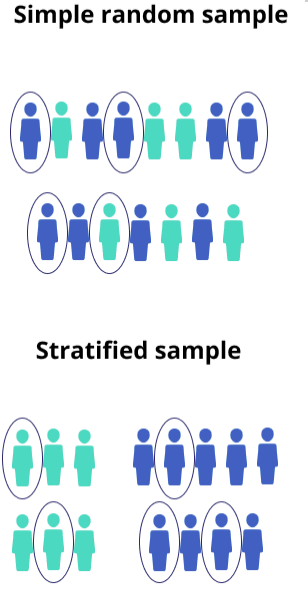
\includegraphics[scale=0.4]{pics/sample_strat.png}
\end{figure}

\footnotemark{Figure source: \url{https://www.scribbr.com/methodology/sampling-methods/}}

} 
\end{frame}



\begin{frame}{A Formal Definition of Statistical Inference }
\scriptsize{
\begin{itemize}
 \item The process of drawing conclusions about a population from sample data is known as \textbf{statistical inference}.
\item From a general point of view, the goal of inference is to \textbf{infer} the distribution that generates the observed data.
\item Example: Given a sample $X_1, \dots, X_n \sim F$, how do we infer $F$? 
\item However, in most cases we are only interested in inferring some property of $F$ (e.g., its \textbf{mean} value).
\item Statistical models that assume that the distribution can be modeled with a finite set of parameters $\theta= (\theta_{1},\theta_{2},\dots,\theta_{k})$ are called \textbf{parametric models}. 
\item Example: if we assume that the data comes from a normal distribution $N(\mu,\sigma^2)$, $\mu$ and $\sigma$ would be the parameters of the model. 
\end{itemize}

} 
\end{frame}


\begin{frame}{Frequentist Aproach}
\scriptsize{
The satistical methods to be presented is this class are known as \textbf{frequentist (or classical)} methods. They are based on the following postulates  \cite{wasserman2013all}:
\begin{itemize}
\item Probability refers to limiting relative frequencies. Probabilities are objective properties of the real world.
\item Parameters are fixed, unknown constants. Because they are not fluctuating, no useful probability statements can be made about parameters.
\item Statistical procedures should be designed to have well-defined long run frequency properties. For example, a 95 percent confidence interval should trap the true value of the parameter with limiting frequency at least 95 percent.
\end{itemize}
There is another approach to inference called \textbf{Bayesian inference}, which is based on different posulates, to be discussed later in the course.

} 
\end{frame}

\section{Point Estimation}

\begin{frame}{Point Estimation}
\scriptsize{
\begin{itemize}
 \item Point estimation is the process of finding the \textbf{best guess} for some quantity of interest from a \textbf{statistical sample}.
 \item In a general sence, this quantity of interest could be a parameter in a parametric model, a CDF $F$, a probability density function $f$, a regression function $r$, or a prediction for a future value $Y$ of some random variable.
 \item In this class we will consider this quantity of interest as a \textbf{population parameter} $\theta$. 
  \item By convention, we denote a point estimate of $\theta$ by $\hat{\theta}$ or $\hat{\theta}_n$.
 \item It is important to remark that while $\theta$ is an unknown fixed value, $\hat{\theta}$  depends on the sample data and is therefore a random variable. 
 \item We need to bear in mind that the process of sampling is by definition a \textbf{random experiment}. 
 
\end{itemize}

} 
\end{frame}

\begin{frame}{Point Estimation}

%http://homepage.divms.uiowa.edu/~rdecook/stat2020/notes/ch7_pt1.pdf

\scriptsize{
\begin{block}{Formal Definition}
\begin{itemize}
 \item Let $X_1, \dots, X_n$ be $n$ IID data points  from some distribution  $F$.
 \item A point estimator $\hat{\theta}_n$  of a parameter $\theta$ is some function of $X_1, \dots, X_n$:
 \begin{displaymath}
 \hat{\theta}_n=g(X_1, \dots, X_n) 
 \end{displaymath}
 
\end{itemize}

 
\end{block}

\begin{itemize}
 \item The \textbf{bias} of an estimator is defined as: 
\begin{displaymath}
 \text{bias}(\hat{\theta}_n)=\mathbb{E}(\hat{\theta}_n)-\theta
\end{displaymath}
\item An estimator is unbiased if $\mathbb{E}(\hat{\theta}_n)=\theta$ or  $\text{bias}(\hat{\theta}_n)=0 $
\end{itemize}

} 
\end{frame}


\begin{frame}{Sampling Distribution}

\scriptsize{
% https://en.wikipedia.org/wiki/Sampling_distribution

\begin{itemize}
\item If we take multiple samples, the value of our statistical estimate $\hat{\theta}_n$ will also vary from sample to sample.

\item We refer to this distribution of our estimator across samples as the   \textbf{sampling distribution} \cite{poldrack2019statistical}.

\item The sampling distribution may be considered as the distribution of  $\hat{\theta}_n$ for all possible samples from the same population of size $n$\footnote{\url{https://courses.lumenlearning.com/boundless-statistics/chapter/sampling-distributions/}}.

\item The sampling distribution describes the variability of the point estimate around the true population parameter from sample to sample. 

\item We need to bear in mind this is an imaginary concept, since in real sitations we can't obtain all possible samples.

\item Actually, in most cases we will only work with a single sample.

\end{itemize}

} 
\end{frame}


\begin{frame}{Standard Error}

\scriptsize{

\begin{itemize}
\item The standard deviation of $\hat{\theta}_n$ is called the \textbf{standard error} $se$:
\begin{displaymath}
se(\hat{\theta}_n)=\sqrt{\mathbb{V}(\hat{\theta}_n})
\end{displaymath}
\item The standard error tells us about the variability of the estimator between all possible samples of the same size.
\item It can be considered as the standard deviation of the sampling distribution. 
\item It is a measure of the uncertainty of the point estimate.
\end{itemize}

} 
\end{frame}





\begin{frame}{The Sample Mean}
\scriptsize{

\begin{itemize}
 \item Let $X_1,X_2,\dots,X_n$ be a random sample of a population of mean $\mu$ and variance $\sigma^2$.
 \item Let's suppose that we are interested in estimating the \textbf{population mean} $\mu$ (e.g., the mean height of Chilean people).
 \item  A sample statistic we can derive from the data is the  \textbf{sample mean} $\overline{X_{n}}$:
 \begin{displaymath}
  \overline{X_{n}}=\frac{1}{n}\sum_{i=1}^{n} X_i
 \end{displaymath}
 \item The sample mean is a \textbf{point estimator} of the mean $\overline{X_{n}} = \hat{\mu}$.

\item We can show that the sample mean is an unbiased estimator of $\mu$:
\begin{displaymath}
\mathbb{E}(\overline{X_{n}}) = \mathbb{E}(\frac 1n \sum_{i=1}^{n} X_i)  =  \frac 1n \times \mathbb{E}(\sum_{i=1}^{n} X_i) = \frac 1n (n \times \mu) = \mu  
\end{displaymath}
\end{itemize}

} 
\end{frame}

\begin{frame}{The Standard Error of the Sample Mean}
\scriptsize{

\begin{itemize}
\item The standard error of the sample mean $se(\overline{X_{n}}) = \sqrt{\mathbb{V}(\overline{X_{n}})}$ can be calulated as:
\begin{displaymath}
 \mathbb{V}(\overline{X_{n}})=\mathbb{V}(\frac 1n \sum_{i=1}^{n} X_i) = \frac{1}{n^2} \mathbb{V}(\sum_{i=1}^{n} X_i) = \frac{n}{n^2} \mathbb{V}(X_i)=\frac{\sigma^2}{n} 
\end{displaymath}

\item Then,
\begin{displaymath}
 se(\overline{X_{n}}) = \frac{\sigma}{\sqrt{n}}
\end{displaymath}





\item The formula for the standard error of the mean implies that the quality of our measurement involves two quantities: the population variability $\sigma$, and the size of our sample $n$.

\end{itemize}


} 
\end{frame}


\begin{frame}{The Standard Error of the Sample Mean}
\scriptsize{

\begin{itemize}
\item We have no control over the population variability, but we do have control over the sample size. 
\item Thus, if we wish to improve our sample statistics (by reducing their sampling variability) then we should use larger samples.
\item However, the formula also tells us something very fundamental about statistical sampling.
\item That the utility of larger samples diminishes with the square root of the sample size. 
\item This means that doubling the sample size will not double the quality of the statistics; rather, it will improve it by a factor of $\sqrt{2}$. \cite{poldrack2019statistical}


\end{itemize}


} 
\end{frame}



\begin{frame}{Sample Variance}
\scriptsize{
\begin{itemize}
 \item A common problem when calculating $ se(\overline{X_{n}})$ is that, in general, we do not know $\sigma$ of the population.
 \item In those cases we can estimate $\sigma$ using the \textbf{sample variance} $s$:
\begin{displaymath}
 s^{2}= \frac{1}{n-1} \sum_{i}^{n}(X_{i}-\overline{X_{n}})^2
\end{displaymath}

\item This is an unbiased estimator of the variance.

\item The standard error of the sample mean when the population variance is unknown can be estimated as follows:
\begin{displaymath}                                                                                                                 
\hat{se}(\overline{X_{n}}) = \frac{s}{\sqrt{n}}                                                                                                                \end{displaymath}


\end{itemize}


} 
\end{frame}



\begin{frame}{Population Variance}
\scriptsize{
\begin{itemize}
\item There is also the population variance, defined as follows:

\begin{displaymath}
 \sigma^{2}= \frac{1}{N} \sum_{i}^{n}(X_{i}-\overline{X_{N}})^2
\end{displaymath}

\item The population variance should only be calculated from population data (all the individuals).

\item Note that we are using $N$ instead of $n$ to denote the entire population rather than a sample.

\item If is calculated from a sample, it would be a \textbf{biased} estimator of the population variance.

\end{itemize}


} 
\end{frame}


\begin{frame}[fragile]{The Sampling Distribution of the Sample Mean}
\scriptsize{

\begin{itemize}
\item We discussed earlier that the sampling distribution is an imaginary concept.
\item Let's imagine the sampling distribution of the sample mean.
\item Imagine drawing (with replacement) all possible samples of size $n$ from a population.
\item Then for each sample, calculate the sample statistic, which is this case is the sample mean. 
\item The frequency distribution of those sample means would be the sampling distribution of the mean (for samples of size $n$ drawn from that particular population).
\item In the next example we will calculate the sampling distribution for a toy example in which the population is known.
\end{itemize}


} 
\end{frame}


\begin{frame}[fragile]{The Sampling Distribution of the Sample Mean}
\scriptsize{
\begin{itemize}
\item Suppose our entire population is a family of 5 siblings and our property of interest is age measured in years.

\item Our population consists of the following 5 values: 2, 3, 4, 5, and 6. 
\item Let's calculate the population mean $\mu$ and the population standard deviation $\sigma$.
\end{itemize}

\begin{verbatim}
> pop <-c(2,3,4,5,6)
> mean(pop)
[1] 4
> sd.p=function(x){sd(x)*sqrt((length(x)-1)/length(x))}
> sd.p(pop)
[1] 1.414214 
\end{verbatim}

$\mu$=4 and $\sigma=1.414214$

} 
\end{frame}

\begin{frame}[fragile]{The Sampling Distribution of the Sample Mean}
\scriptsize{
\begin{itemize}
\item Now, we will use the R library ``gtools'' to draw all 25 possible samples (with replacement) of size $2$.
\end{itemize}

\begin{verbatim}
> library(gtools)
> library(tidyverse)
> samp_size <- 2
> samples<-as_tibble(permutations(length(pop), samp_size,
+                                 pop, repeats.allowed=TRUE))
> samples
# A tibble: 25 x 2
      V1    V2
   <dbl> <dbl>
 1     2     2
 2     2     3
 3     2     4
 4     2     5
 5     2     6
 6     3     2
 7     3     3
 8     3     4
 9     3     5
10     3     6
# … with 15 more rows
\end{verbatim}



} 
\end{frame}


\begin{frame}[fragile]{The Sampling Distribution of the Sample Mean}
\scriptsize{
\begin{itemize}
\item We can calculate the sample mean of each sample using the command ``mutate'':
\end{itemize}

\begin{verbatim}
> samples <- samples %>% rowwise() %>% 
+   mutate(sample_mean=mean(c(V1,V2)))
> samples
# A tibble: 25 x 3
# Rowwise: 
      V1    V2 sample_mean
   <dbl> <dbl>       <dbl>
 1     2     2         2  
 2     2     3         2.5
 3     2     4         3  
 4     2     5         3.5
 5     2     6         4  
 6     3     2         2.5
 7     3     3         3  
 8     3     4         3.5
 9     3     5         4  
10     3     6         4.5
# … with 15 more rows
\end{verbatim}



} 
\end{frame}



\begin{frame}[fragile]{The Sampling Distribution of the Sample Mean}
\scriptsize{
\begin{itemize}
\item The distribution of these sample means is the \textbf{sampling distributiion}.
\item We can visualize its shape by plotting an histogram: 
\begin{verbatim}
ggplot(samples, aes(x=sample_mean)) + 
  geom_histogram(bins = 10, color="black", fill="white")
\end{verbatim}


\end{itemize}

\begin{figure}[h!]
	\centering
	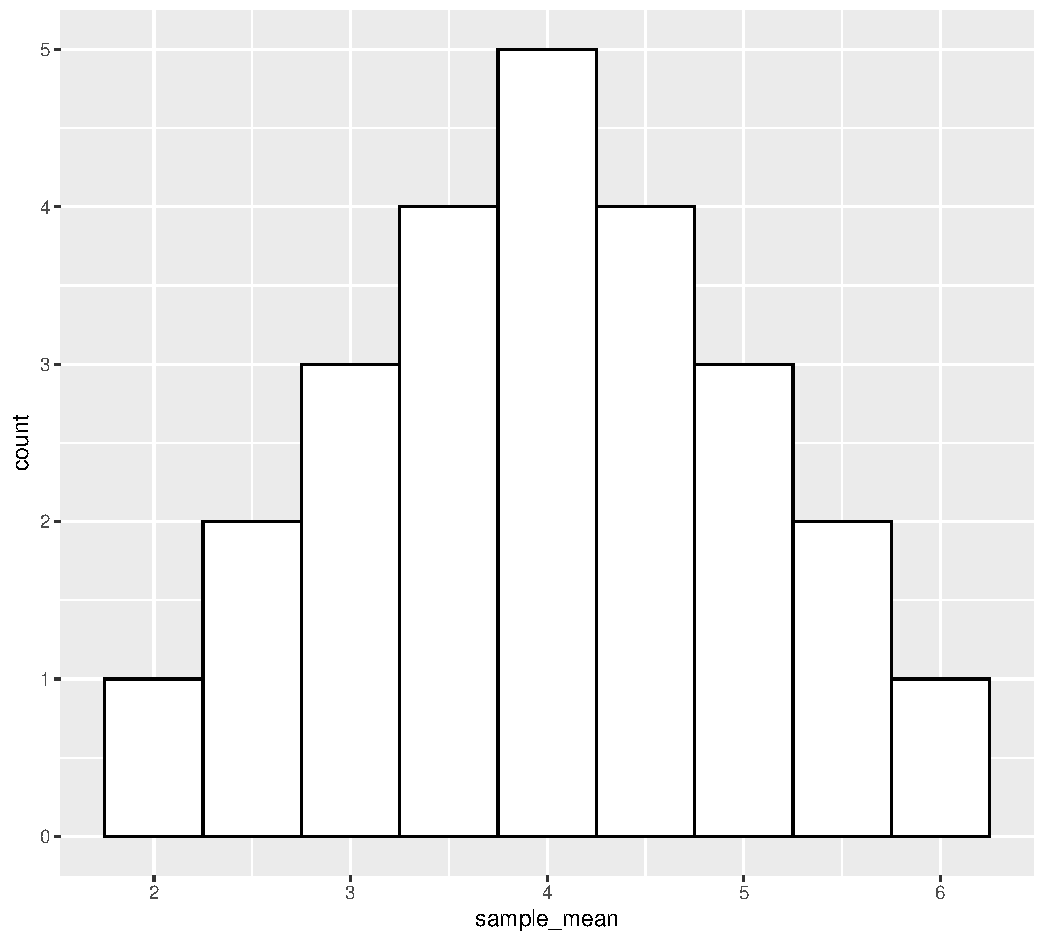
\includegraphics[scale=0.35]{pics/hist_sampdist.pdf}
\end{figure}


} 
\end{frame}


\begin{frame}[fragile]{The Sampling Distribution of the Sample Mean}
\scriptsize{
\begin{itemize}
\item You may noticed that the historgram is peaked in the middle, and symmetrical.
\item This is a consequence of the Central Limit Theorem!!!
\item We can see that the population distribution is very different from the sampling distribution:
\begin{verbatim}
ggplot(data.frame(pop), aes(x=pop)) +
  geom_histogram(bins = 5, color="black", fill="white")
\end{verbatim}


\end{itemize}

\begin{figure}[h!]
	\centering
	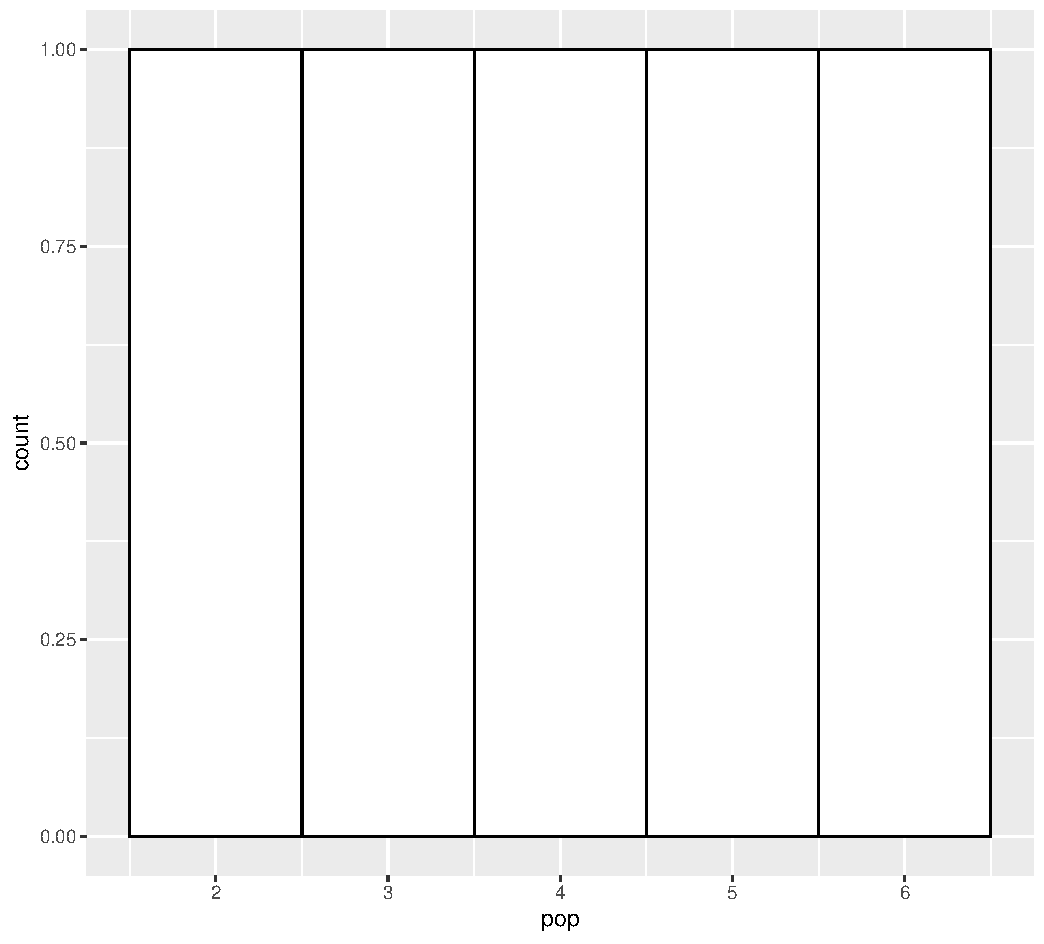
\includegraphics[scale=0.3]{pics/pop_dist.pdf}
\end{figure}




} 
\end{frame}


\begin{frame}[fragile]{The Sampling Distribution of the Sample Mean}
\scriptsize{
\begin{itemize}
\item Let's calculate the mean and the standard deviation of the sample means:
\begin{verbatim}
> mean(samples$sample_mean)
[1] 4
> sd.p(samples$sample_mean)
[1] 1
\end{verbatim}

\item We can see that mean of the sampling distribution of the mean $\mu_{\overline{X}}$ equals the population mean $\mu$.


\item We can also calculate the theoretical standard error $se=\sigma/\sqrt{n}$

\begin{verbatim}
> sd.p(pop)/sqrt(samp_size)
[1] 1
\end{verbatim}

which is the same as the standard distribution of the sampling distribution of the sample mean.

\item We have validated empirically that the sample mean is a good estimator of the population mean and that its standard error can be calculated from the population standard deviation and the sample size.

\end{itemize}



} 
\end{frame}


\begin{frame}[fragile]{The Sampling Distribution of the Sample Mean}
\scriptsize{

\begin{itemize}
\item The central limit theorem tell us the conditions under which the sampling distribution of the mean is normally distributed or at least approximately normal.
\item If the population from which you sample is itself normally distributed, then the sampling distribution of the mean will be normal, regardless of sample size.
\item If the population from which you sample is non-normal, the sampling distribution of the mean will still be approximately normal given a large enough sample size.
\item What size is sufficient? Some authors say 30 or 40. But if the population distribution is extremely non-normal (i.e. very skewed) you will need more.
\end{itemize}


} 
\end{frame}


\begin{frame}{Point Estimation of a Proportion}
\scriptsize{
\begin{itemize}
 \item Suppose we want to estimate the fraction of people who will vote for a certain candidate.
 \item Our population parameter $p$ corresponds to the true fraction of voters for this candidate.
 \item We can model a sample of independent voters  $X_1, \dots, X_n$, as Bernoulli distributed random variables with parameter $p$.
 
 \item  We interpret $X_i=0$ as a negative vote and $X_i=1$ as a positive vote.
 
 \item The sample proportion $\hat{p}_{n}=\frac 1n \sum_{i}X_{i}$ is our estimator of $p$.
\end{itemize}


} 
\end{frame}


\begin{frame}{Point Estimation of a Proportion}
\scriptsize{
\begin{itemize}
 \item Then $\mathbb{E}(\hat{p}_{n})= \frac 1n \sum_i \mathbb{E}(X_i)=p$, and $\hat{p}_n$ is unbiased.
 \item The standard error $se$ would be
\begin{displaymath}
se = \sqrt{\mathbb{V}(\hat{p}_n)}= \sqrt{p(1-p)/n} 
\end{displaymath}
\item The estimated standard error $\hat{se}$:
\begin{displaymath}
\hat{se} =\sqrt{\hat{p}(1-\hat p)/n} 
\end{displaymath}
\item By the Central Limit Theorem the sampling distribution of the sample proportion converges to a Normal distribution: $\hat{p}_{n} \approx N(p, \hat{se}^2)$.

\item This is because the sample proportion is actually the sample mean of a binary population.
\end{itemize}


} 
\end{frame}

\begin{frame}{Consistency}

\scriptsize{

\begin{itemize}
\item A good estimator is expected to be unbiased and of minimum standard error.

\item Unbiasedness used to receive much attention but these days is considered less important

\item Many of the estimators we will use are biased. 

\item A reasonable requirement for an estimator is that it should converge to the true parameter value as we collect more and more data.

\item A point estimator $\hat{\theta}_n$ of a parameter $\theta$ is \textbf{consistent}  if it converges to the true value when the number of data in the sample tends to infinity.

\end{itemize}

} 
\end{frame}



\begin{frame}{Consistency}

\scriptsize{

\begin{itemize}
\item Theorem: If for an estimator $\hat{\theta}_n$, its $bias \rightarrow 0$ and its $se \rightarrow 0$ when $n\rightarrow \infty$, $\hat{\theta}_n$, it is a consistent estimator of $\theta$.

\item For example, for the sample mean $\mathbb{E}(\overline{X_{n}})=\mu$,  which implies that the $bias =0$.
\item Then $se(\overline{X_{n}}) = \frac{\sigma}{\sqrt{n}}$  converges to zero when $n\rightarrow \infty$. 
\item  $\overline{X_{n}}$ is a consistent estimator of the mean.  

\item For the case of the Bernoulli experiment one has that  $\mathbb{E}(\hat{p})=p \Rightarrow bias=0$ and $se = \sqrt{p(1-p)/n} \rightarrow 0$ when $n\rightarrow \infty$. 

\item Then  $\hat{p}$ is a consistent estimator of $p$.


\end{itemize}

} 
\end{frame}


\begin{frame}{Maximum Likelihood Estimation}
\scriptsize{
\begin{itemize}
 \item The estimators we have presented so far (e.g., the sample mean, the sample proportion) are ituitive, easy to compute, and consistent.
 \item Maximum Likelihood Estimation (MLE) is a more general framework  for estimating the \textbf{parameters} of any \textbf{parametric model}.
 \item In MLE, we assume that the sample data is generated by a given probability distribution ( continuous or discrete) parameterized by $\theta$ and try to find the value of $\theta$ that maximizes the joint probability of the data under that distribution. 
 \item Idea: find the parameter values of the assumed statistical model that make the observed data most probable.
 \item For example, we can asssume that each data point is generated by $N(\mu,\sigma^2)$, then we compute the joint PDF (or PMF) of our data and find the parameter values for $\mu$ and $\sigma$ that maximize that joint density (or mass).
 
\end{itemize}


} 
 
\end{frame}

\begin{frame}{Maximum Likelihood Estimation}
\scriptsize{
\begin{itemize}
 \item Students learning statistics often ask: how would we ever know that the distribution that generated the data is in some parametric model? \cite{wasserman2013all}
 \item There are  cases where background knowledge suggests that a parametric model provides a reasonable approximation. 
 \item Example 1: independent binary experiments (e.g., flipping a coin or voting for a candidate) can be adequately represented with Bernoulli or Binomial distributions.
 \item Example 2: counts of traffic accidents are known from prior experience to follow approximately a Poisson model.  
 
 \item  In many other cases non parametric methods are preferable, but they are beyond the scope of this course.
 
\end{itemize}


} 
 
\end{frame}



\begin{frame}{Maximum Likelihood Estimation}
\scriptsize{
\begin{itemize}
 \item Let $X_1,\dots,X_n$ be IID with PDF (or PMF) $f(x;\theta)$.
 \item Since we are assuming that our data samples are independent random variables, the joint density (or mass) would be the product of each PDF (or PMF): 
 \begin{displaymath}
\mathcal{L}_{n}(\theta)=\prod_{i=1}^nf(X_i;\theta)  
 \end{displaymath}
\item We refer to this joint density (or mass) as the \textbf{likelihood function}.
\item The likelihood function is just the joint density (or mass) of the data, except that we treat it is a function of the parameter $\theta$.

\item In MLE, we turn the estimation task into an optimization problem:

\begin{center}
\begin{equation}
\begin{split}
\max_{\theta} & \quad \mathcal{L}_{n}(\theta)
\end{split}
\end{equation}
\end{center}

\item The maximum likelihood estimator MLE, denoted by $\hat{\theta}_n$, is the value of $\theta$ that maximizes $\mathcal{L}_{n}(\theta)$.
 
\end{itemize}


} 
 
\end{frame}


\begin{frame}{Maximum Likelihood Estimation}
\scriptsize{
\begin{itemize}
 \item In many cases the log-likelihood is easier to optimize $l_n(\theta)$:
 
 \begin{displaymath}
l_n(\theta) = \log(\mathcal{L}_{n}(\theta))=\log(\prod_{i=1}^nf(X_i;\theta))= \sum_{i=1}^{n}\log(f(X_i;\theta))  
 \end{displaymath} 

\item Since the logarithm is a monotonic function, the maximum of occurs at the same value of $\theta$.
 
\item If the $l_n$ is differentiable we can find   $\hat{\theta}_n$ by setting the derivatives to zero:

\begin{displaymath}
 \frac{\partial l_n}{\partial \theta} = 0
\end{displaymath}

\item The MLE has many good mathematical properties that go beyond the scope of this course to discuss.

\item One property that is important to know is that the MLE is \textbf{consistent}.

\end{itemize}


} 
 
\end{frame}


\begin{frame}{Maximum Likelihood Estimation}
\scriptsize{
\begin{itemize}
 \item Example 1: Suppose that $X_1,\dots, X_n \sim$  Bernoulli$(p)$. 
 \item The probability mass function is $f(x;p)= p^x(1- p)^{1-x}$ for $x = 0,1$. The unknown parameter is $p$. 
 \item Then,
 
 \begin{displaymath}
\mathcal{L}_{n}(p)=\prod_{i=1}^nf(X_i;p) = \prod_{i=1}^np^{X_i}(1-p)^{1-X_i}=p^S(1-p)^{n-S} 
 \end{displaymath} 
where $S=\sum_{i}X_i$. Hence, 
 
 \begin{displaymath}
l_n(\theta) = S\log p+ (n-S)\log(1-p). 
 \end{displaymath}  
 
\item Take the derivative of $l_n(\theta)$, set it equal to 0 to find that the MLE is $\hat{p}_n =S/n$, which is the sample proportion.
 
\end{itemize}


} 
 
\end{frame}

\begin{frame}{Maximum Likelihood Estimation}
\scriptsize{
\begin{itemize}
 \item Example 2: Let  $X_1,\dots, X_n \sim N(\mu,\sigma^2)$. 
 \item The parameter is $\theta=(\mu,\sigma)$ and the likelihood function (ignoring some constants) is:
 
 
  \begin{align}
\mathcal{L}_{n}(\mu,\sigma) & =\prod_{i=1}^n \frac{1}{\sigma} \exp \left( - \frac{1}{2\sigma^2} (X_i -\mu)^2 \right) \\
 & = \frac{1}{\sigma^n}\exp \left( - \frac{1}{2\sigma^2} \sum_{i=1}^n(X_i -\mu)^2 \right) \\
  & = \frac{1}{\sigma^n}\exp \left( - \frac{nS^2}{2\sigma^2} \right)\exp \left( - \frac{n(\overline{X}-\mu)^2}{2\sigma^2} \right)
 \end{align}

\item Where $\overline{X}=\frac{1}{n}\sum_{i=1}^nX_i$ is the sample mean and $S^2 = \frac{1}{n}\sum_{i=1}^n(X_i-\overline{X}^2)$.
\end{itemize}
} 
 
\end{frame}



\begin{frame}{Maximum Likelihood Estimation}
\scriptsize{
\begin{itemize}
\item The last equality above follows from the fact that 
\begin{displaymath}
 \sum_{i=1}^n(X_i -\mu)^2=nS^2+n(\overline{X}-\mu)^2
\end{displaymath}

which can be verified by writing
\begin{displaymath}
\sum_{i=1}^n(X_i -\mu)^2 = \sum_{i=1}^n(X_i - \overline{X} + \overline{X} -\mu)^2 
\end{displaymath}
and then expanding the square.
 
\item The log-likelihood is: 
 
 \begin{displaymath}
l_n(\mu,\sigma) = -n\log \sigma - \frac{nS^2}{2\sigma^2} - \frac{n(\overline{X}-\mu)^2}{2\sigma^2} 
 \end{displaymath}   

 
\item Solving the equations $\frac{\partial (\mu,\sigma)}{\partial \mu} = 0$ and $\frac{\partial (\mu,\sigma)}{\partial \sigma} = 0$

\item We conclude that $\hat{\mu} = \overline{X}$ and $\hat{\sigma}=S$. 

\item It can be verified that these are indeed global maxima of the likelihood.

\end{itemize}



} 
 
\end{frame}


\begin{frame}{Confidence Interval}
\scriptsize{
\begin{itemize}
 \item We know that the value of a point estimator \textbf{varies} from sample to sample.
 \item It is more reasonable to find an interval that is likely to trap the real value of the parameter in the long run.
 \item The general form of a confidence interval in the following:
  \begin{displaymath}
   \text{Confidence Interval} = \text{Sample Statistic} \ \pm \ \text{Margin Error}
  \end{displaymath}
 \item The wider the interval the more uncertainty there is about the value of the parameter.
\end{itemize}


}
 
\end{frame}


\begin{frame}{Confidence Interval }
\scriptsize{

\begin{block}{Definition}
\begin{itemize}
 \item A \textbf{confidence interval} for an unknown population parameter $\theta$ with a \textbf{confidence level} $1-\alpha$, is an interval $C_n = (a,b)$ where:
 \begin{displaymath}
 \mathbb{P}(\theta \in C_n) = 1-\alpha
\end{displaymath}
 \item In addition $a= a(X_1, \dots, X_n)$ and $b=b(X_1,\dots,X_n)$ are functions of the data.
 \item The $\alpha$ value is known as the \textbf{significance} level, generally taken as $0.05$, which is equivalent to working with a confidence level of $95\%$.
 \item Significance can be interpreted as the probability of being wrong.
\end{itemize}

\end{block}

}
 
\end{frame}


\begin{frame}{Confidence Interval}
\scriptsize{


\begin{itemize}
 \item There is a lot of \textbf{confusion} about how to interpret a confidence interval.
 \item A confidence interval is not a probability statement about $\theta$ since $\theta$ is a fixed quantity in frequentist inference, not a random variable
 \item One way to interpret them is to say that if we repeat the \textbf{same experiment} many times, the interval will contain the value of the parameter $(1-\alpha)\%$ of the times.
 \item This interpretation is correct, but we rarely repeat the same experiment several times.
 \item A better interpretation: one day I collect data I create a $95\%$ confidence interval for a parameter $\theta_1$. Then on day 2, I do the same for a parameter $\theta_2$ and so repeatedly $n$ times. The $95\%$ of my intervals will contain the actual values of the parameters. 
 
\end{itemize}



}
 
\end{frame}




\begin{frame}{Confidence Interval}
\scriptsize{


\begin{itemize}
 \item Later in the course, we will discuss Bayesian methods in which we treat $\theta$ as if it were a random variable and we do make probability statements about $\theta$.
\item In particular, we will make statements like ``the probability that $\theta$  is in $C_n$, given the data, is 95 percent.''
\item However, these Bayesian intervals refer to degree-of-belief probabilities. 
\item These Bayesian intervals will not, in general, trap the parameter 95 percent of the time.
 
\end{itemize}



}
 
\end{frame}


\begin{frame}{Confidence Interval of the Mean }
\scriptsize{
\begin{itemize}
 \item We have $n$ independent observations $X_1, \dots, X_n$ (IID) of distribution $N(\mu,\sigma^2)$.
\item Suppose $\mu$ is \textbf{unknown} but $\sigma^2$ is \textbf{known}.
 \item We know that $\overline{X_{n}}$ is an unbiased estimator of $\mu$.
 \item By the law of large numbers we know that the distribution of $\overline{X_{n}}$ is concentrated around $\mu$ when $n$ is large.
 \item By the CLT we know that \begin{displaymath}
 Z=\frac{\overline{X_{n}}-\mu}{\frac{\sigma}{\sqrt{n}}}  \sim N(0,1)
\end{displaymath}
when $n$ is large.
\end{itemize}


 }
\end{frame}

\begin{frame}{Confidence Interval}
\scriptsize{
\begin{itemize}
 \item We want to find an interval $C_n = (\mu_1,\mu_2)$ with confidence level $1-\alpha$:
\begin{displaymath}
 \mathbb{P}(\mu_1 \leq \mu \leq \mu_2 ) = 1-\alpha
\end{displaymath}
\item Let $z_a = \Phi^{-1}(1-a)$, with $a \in [0,1]$ where $\Phi^{-1}$ is the quantile function of a standardized normal.
\item This is equivalent to saying that $z_a$ is the value such that $1-\Phi(z_a)=\mathbb{P}(Z \geq z_a)=a$.

\item By symmetry of the normal distribution: $z_{\alpha/2}=-z_{(1-\alpha/2)}$.
\end{itemize}


 }
\end{frame}



\begin{frame}{Confidence Interval}


\begin{figure}[h!]
	\centering
	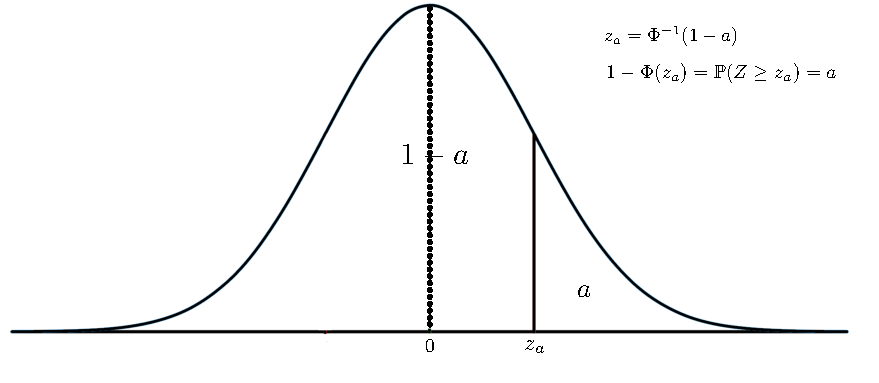
\includegraphics[scale=0.8]{pics/conf_int_1.pdf}
\end{figure}


 
\end{frame}


\begin{frame}{Confidence Interval}


\begin{figure}[h!]
	\centering
	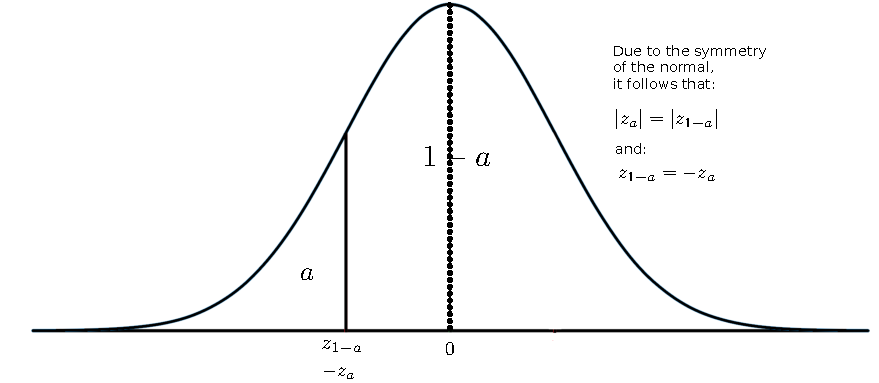
\includegraphics[scale=0.8]{pics/conf_int_2.pdf}
\end{figure}


 
\end{frame}


\begin{frame}{Confidence Interval}


\begin{figure}[h!]
	\centering
	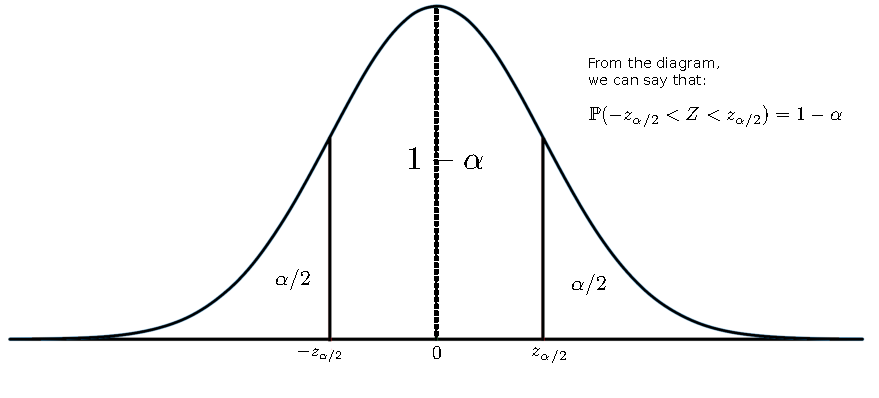
\includegraphics[scale=0.8]{pics/conf_int_3.pdf}
\end{figure}


 
\end{frame}


\begin{frame}{Confidence Interval}
\scriptsize{
\begin{itemize}
 \item  The confidence interval for $\mu$ is:
 \begin{displaymath}
 C_n = (\overline{X_{n}}-z_{\alpha/2}\frac{\sigma}{\sqrt{n}} , \overline{X_{n}} + z_{\alpha/2}\frac{\sigma}{\sqrt{n}}) 
 \end{displaymath}
\item Then $ z_{\alpha/2}$ tells us how many times we have to multiply the \textbf{standard error} to build the interval.
\item The smaller the value of $\alpha$ the larger the value of $ z_{\alpha/2}$ and hence the wider the interval.  
\item Proof:
 \begin{eqnarray*}
 \mathbb{P}(\mu \in C_n) & = & \mathbb{P}(\overline{X_{n}}-z_{\alpha/2}\frac{\sigma}{\sqrt{n}} < \mu < \overline{X_{n}} + z_{\alpha/2}\frac{\sigma}{\sqrt{n}}) \nonumber \\ 
                         & = & \mathbb{P}(-z_{\alpha/2} < \frac{\overline{X_{n}}-\mu}{\frac{\sigma}{\sqrt{n}}} <  z_{\alpha/2}) \nonumber \\ 
			  & = & \mathbb{P}(-z_{\alpha/2} < Z <  z_{\alpha/2}) \nonumber \\
			   & = & 1-\alpha 
 \end{eqnarray*}


\end{itemize}
}


 
\end{frame}

\begin{frame}[fragile]{Confidence Interval}

\scriptsize{
\begin{itemize}
 \item Since $z_{\alpha/2} = \Phi^{-1}(1-\alpha/2)$ we can use the quantile function of the normal to calculate confidence intervals in R.
\end{itemize}


\begin{verbatim}
> alpha <- 0.05
> xbar <- 5
> sigma <- 2
> n <- 20
> se <-sigma/sqrt(n)
> error <- qnorm(1-alpha/2)*se
> left <- xbar-error
> right <- xbar+error
> left
[1] 4.123477
> right
[1] 5.876523
>
\end{verbatim}
}



\end{frame}

\begin{frame}{T Distribution}
\scriptsize{
\begin{itemize}
 \item In practice, if we do not know $\mu$ we are unlikely to know $\sigma$.
 \item If we estimate $\sigma$ using $s$, confidence intervals are better build using the \textbf{T-student} distribution, especially when the sample size is small.
\end{itemize}

\begin{block}{T Distribution}
\begin{itemize}
 \item An R.V. has distribution $t$ with $k$ degrees of freedom when it has the following PDF:
\begin{displaymath}
 f(t)=\frac{\Gamma(\frac{k+1}{2})}{\sqrt{k\pi}\Gamma(\frac k2)(1+\frac{t^2}{k})^{(k+1)/2}}
\end{displaymath}
\item  When $k=1$ it is called \textbf{Cauchy} distribution.
\item When $k\rightarrow \infty$ it converges to a standardized normal distribution.
 \item The t-distribution has wider tails than the normal distribution when it has few degrees of freedom.


\end{itemize}

 
\end{block}




} 
\end{frame}

\begin{frame}[fragile]{T Distribution}
 \scriptsize{



\begin{verbatim*}
x<-seq(-8,8,length=400)
y1<-dnorm(x)
y2<-dt(x=x,df=1)
y3<-dt(x=x,df=10)
y4<-dt(x=x,df=350)
plot(y1~x,type="l",col="green")
lines(y2~x,type="l",col="blue")
lines(y3~x,type="l",col="black")
lines(y4~x,type="l",col="red")

\end{verbatim*}

 \begin{figure}[h!]
	\centering
	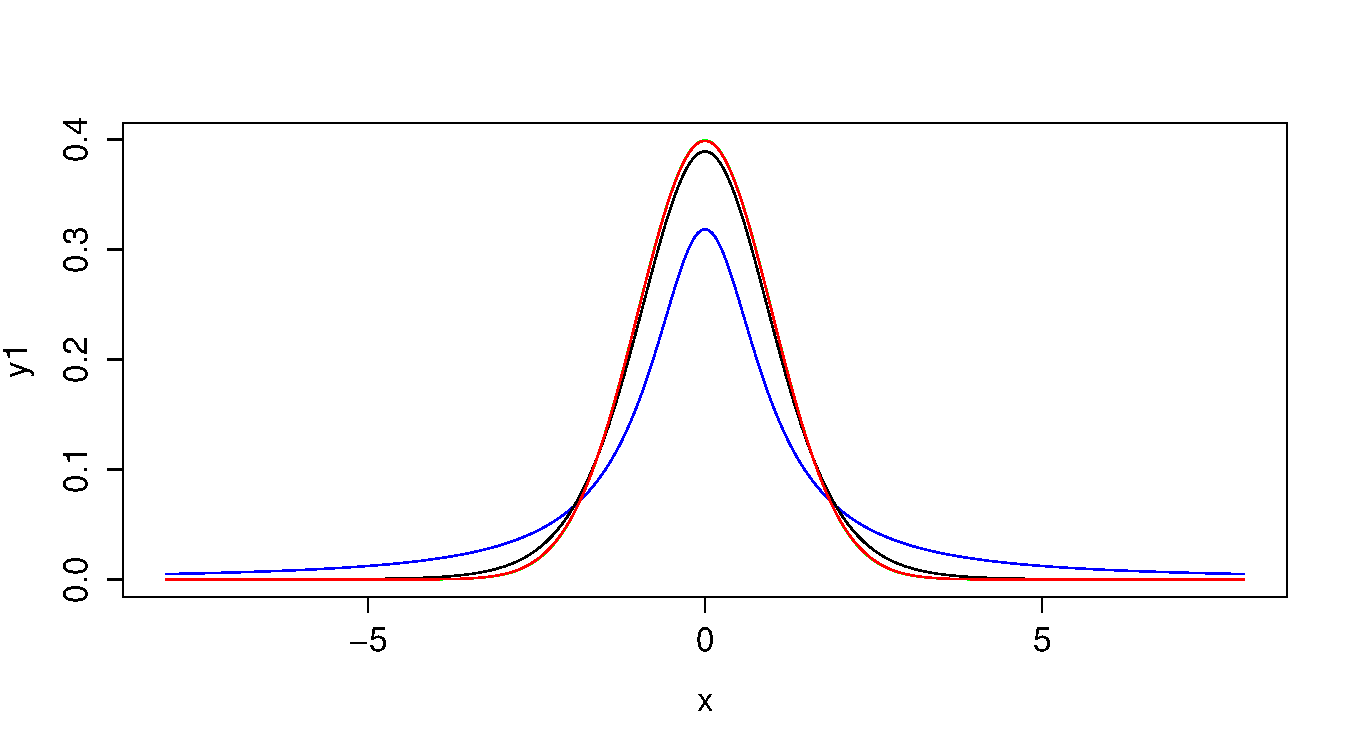
\includegraphics[scale=0.3]{pics/tstudent.pdf}
\end{figure}


}
\end{frame}


\begin{frame}{T-Distribution Confidence Interval}

\scriptsize{
\begin{itemize}
 \item Let  $s^{2}= \frac{1}{n-1} \sum_{i}^{n}(X_{i}-\overline{X_{n}})^2$ we have:
 \begin{displaymath}
  T=\frac{\overline{X_{n}}-\mu}{\frac{s}{\sqrt{n}}}\sim t_{n-1}
 \end{displaymath}
\item  Let $t_{n-1,a}=\mathbb{P}(T>a)$, equivalent to the quantile function $qt$ evaluated at $(1-a)$.
\item The resulting confidence interval is:
       \begin{displaymath}
 C_n = (\overline{X_{n}}-t_{n-1,\alpha/2}\frac{s}{\sqrt{n}} , \overline{X_{n}} + t_{n-1,\alpha/2}\frac{s}{\sqrt{n}}) 
 \end{displaymath} 
 \item Since the tails of the $t$ distribution are wider when $n$ is small, the resulting confidence intervals are wider.

\end{itemize}


}

\end{frame}


\begin{frame}[fragile]{T-Distribution Confidence Interval}
\scriptsize{
\begin{itemize}
 \item Let's calculate a confidence interval for the mean of \verb+Petal.Length+ of the \textbf{Iris} data with $95\%$ confidence.
\begin{verbatim}
>data(iris)
>alpha<-0.05
>n<-length(iris$Petal.Length)
>xbar<-mean(iris$Petal.Length)
>xbar
[1] 3.758
>s<-sd(iris$Petal.Length)
>se<-s/sqrt(n)
>error<-qt(p=1-alpha/2,df=n-1)*se
>left<-xbar-error
>left
[1] 3.473185
>right<-xbar+error
>right
[1] 4.042815
\end{verbatim}
\item Another way:
\begin{verbatim}
>test<-t.test(iris$Petal.Length,conf.level=0.95)
>test$conf.int
[1] 3.473185 4.042815
\end{verbatim}


\end{itemize}


}
\end{frame}

\begin{frame}{Confidence Interval for a Population Proportion}
\scriptsize{
\begin{itemize}
 \item Suppose we want to compute the proportion of subjects who will vote for a candiate and we also want a confidence interval for the estimated proportion.
 
 \item As showed earlier, the sampling distribution of a the sample proportion follows a Normal distribution.

 \item The confidence interval $C_n$ for a proportion is:
\begin{displaymath}
 C_n = \left(\hat{p}-z_{\alpha/2}\sqrt{\frac{\hat{p}(1-\hat p)}{n}} , \hat{p} + z_{\alpha/2}\sqrt{\frac{\hat{p}(1-\hat p)}{n}}\right) 
 \end{displaymath} 



\end{itemize}

}

 
\end{frame}


\begin{frame}[fragile]{Confidence Interval for a Population Proportion}
\scriptsize{
\begin{itemize}
\item Example: $1,219$ respondents indicated that they would vote for candidate A in a survey of $3,532$ people. 

\item Compute a 95\% confidence interval for the proportion of voters: 
 
\begin{displaymath}
 \hat{p}=\frac{1219}{3235}=0.345
\end{displaymath}

\item and $z_{\alpha/2}=1.96$ 
\begin{verbatim}
> qnorm(1-0.025)
[1] 1.959964
\end{verbatim}

\begin{displaymath}
 C_n = 0.345 \pm 1.96\sqrt{\frac{0.345(1-0.345)}{3532}} = (0.329,0.361)  
 \end{displaymath} 
 
\item In R:
 
\begin{verbatim}
> prop<-prop.test(1219,3532,correct=FALSE)
> prop$conf.int
[1] 0.3296275 0.3609695
\end{verbatim}



\end{itemize}

}

 
\end{frame}



\begin{frame}{The Boostrap}
\scriptsize{

\begin{itemize}
 \item We have used our knowledge of the sampling distribution of the mean to compute the standard error of the mean. 
 \item But what if we can't assume that the estimates are normally distributed, or we don’t know their distribution? 
 \item The idea of the bootstrap is to use the data themselves to estimate an answer. 
 \item The bootstrap method was conceived by Bradley Efron of the Stanford Department of Statistics, who is one of the world's most influential statisticians.
\item The idea behind the bootstrap is that we repeatedly sample from the actual dataset.

\item We sample with replacement, such that the same data point will often end up being represented multiple times within one of the samples. 

\end{itemize}
}
 
\end{frame}

\begin{frame}{The Boostrap}
\scriptsize{

\begin{itemize}

\item We then compute our statistic of interest on each of the bootstrap samples, and use the distribution of those estimates as our sampling distribution. 



\item In a sense, we treat our particular sample as the entire population, and then repeatedly sample with replacement to generate our samples for analysis.
\item This makes the assumption that our particular sample is an accurate reflection of the population, which is probably reasonable for larger samples but can break down when samples are smaller.

\item This technique can be used to estimate the standard error of any statistic and to obtain a confidence interval (CI) for it. 



\end{itemize}
}
 
\end{frame}



\begin{frame}{The Boostrap}
\scriptsize{

\begin{itemize}
\item Let's use the bootstrap to estimate the sampling distribution of the mean:

\begin{figure}[h!]
	\centering
	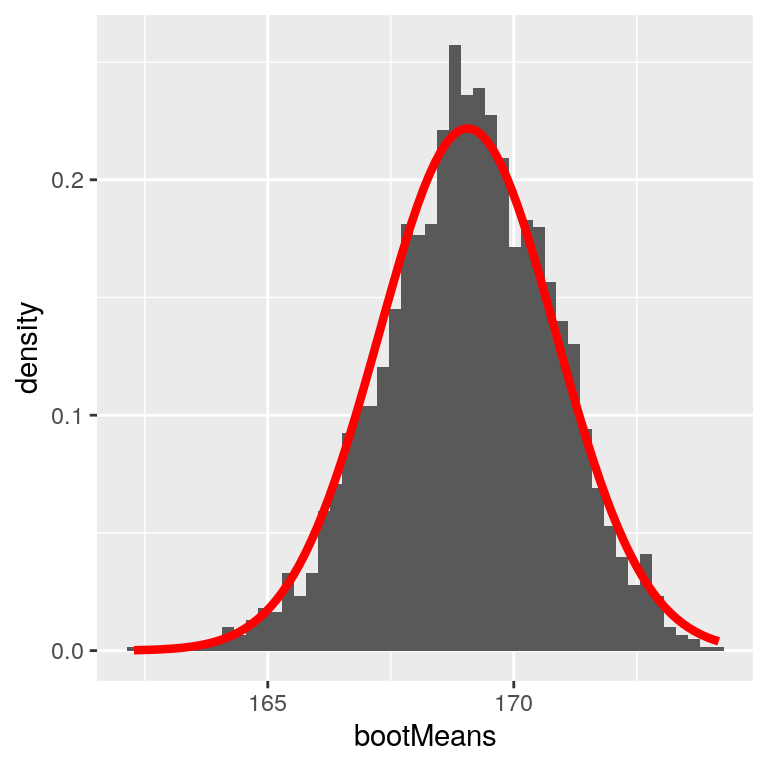
\includegraphics[scale=0.5]{pics/bootstrapSEM-1.png}
\end{figure}

\item The histogram shows the distribution of means across bootstrap samples, while the red line shows the normal distribution based on the sample mean and standard error. 

\end{itemize}
}
 
\end{frame}



\begin{frame}{The Boostrap}
\scriptsize{

\begin{itemize}
\item From the figure, we can see that the distribution of means across bootstrap samples is fairly close to the theoretical estimate based on the assumption of normality. 

\item It doesn't make much sense to use bootstrap for the sample mean because we know the theoerical shape of the sampling distribution.

\item The bootstrap would more often be used to generate standard errors and confidence intervals for estimates of statistics (e.g., the median, the maximum) where we know or suspect that the normal distribution is not appropriate. 

\item Bootstrap is especially useful when CI doesn't have a closed form, or it has a very complicated one.

\item Tutorials: \url{https://www.datacamp.com/community/tutorials/bootstrap-r}, \url{https://github.com/statsthinking21/statsthinking21-R/blob/master/07-ResamplingAndSimulation.Rmd}.

\end{itemize}
}
 
\end{frame}



\begin{frame}{Conclusions}
\scriptsize{

\begin{itemize}
\item We have introduced many important concepts in statistical inference, in particular, the frequentist approach.

\item We have studied estimators and their sampling distributions.

\item We introduced a general technique for calculating estimators called maximum likelihood.

\item We studied how to measure the uncertainty of an estimator using a confidence interval.

\item We have introduced a method of approximating confidence intervals by means of simulations called bootstrap.

\end{itemize}
}
 
\end{frame}


%%%%%%%%%%%%%%%%%%%%%%%%%%%
%%%%%%%%%%%%%%%%%%%%%%%%%%%
\begin{frame}[allowframebreaks]\scriptsize
\frametitle{References}
\bibliography{bio}
\bibliographystyle{apalike}
%\bibliographystyle{flexbib}
\end{frame}  








%%%%%%%%%%%%%%%%%%%%%%%%%%%

\end{document}
